\documentclass[10pt,twocolumn]{article}

\usepackage[a4paper,margin=0.72in]{geometry}
\usepackage[T1]{fontenc}
\usepackage{lmodern}
\usepackage{microtype}
\usepackage{amsmath,amssymb}
\usepackage{booktabs}
\usepackage{tabularx}
\usepackage{graphicx}
\usepackage{caption}
\usepackage{subcaption}
\usepackage{algorithm}
\usepackage{algpseudocode}
\usepackage[numbers,sort&compress]{natbib}
\usepackage{xurl}
\usepackage{hyperref}

\hypersetup{
  colorlinks=true,
  linkcolor=black,
  citecolor=blue,
  urlcolor=blue
}

\graphicspath{{figures/}}
\newcommand{\cmaps}{C-MAPSS}
\newcommand{\rul}{RUL}

\title{\textbf{Safety-Aware Evaluation and Improvement of Classical and Deep Sequence Models for Turbofan Engine RUL Prediction on C-MAPSS}}
\author{Ethan Huang\\Beihang University}
\date{June 25, 2026}

\begin{document}
\maketitle

\begin{abstract}
Remaining useful life (RUL) estimation is a core prognostics and health management task for aero-engine maintenance. Recent C-MAPSS studies often compare classical regressors, convolutional models, and recurrent neural networks primarily through aggregate accuracy. This paper revisits that benchmark setting from a safety-aware perspective. Using the NASA C-MAPSS FD001 and FD003 subsets, we compare Ridge regression, Random Forest, Gradient Boosting, LSTM, GRU, and 1D-CNN pipelines under leakage-controlled preprocessing, engine-level validation splitting, capped RUL labels, and three random seeds. We further evaluate focused GRU variants, including longer temporal windows, larger hidden capacity, learning-rate changes, and lightweight safety-aware losses that upweight late-life samples and overestimation errors. Results show that tree ensembles remain strong on the simpler FD001 subset, while a 50-cycle GRU obtains the numerically lowest FD003 RMSE among the evaluated configurations; a paired bootstrap comparison with Gradient Boosting is not statistically resolved. More importantly, model ranking changes under safety-oriented metrics: safety-weighted GRUs improve FD001 critical-zone RMSE and reduce FD003 overestimation frequency, even when they do not dominate aggregate RMSE. The study argues that C-MAPSS RUL reports should include critical-zone error and overestimation behavior alongside RMSE, MAE, and NASA score. The contribution is scoped as a reproducible student research benchmark rather than a new state-of-the-art method.
\end{abstract}

\noindent\textbf{Keywords:} remaining useful life; prognostics and health management; C-MAPSS; turbofan engine; safety-aware learning; GRU

\section{Introduction}

Remaining useful life (RUL) prediction estimates how many operating cycles remain before a component reaches failure. In prognostics and health management (PHM), accurate RUL estimation supports maintenance scheduling, fleet availability, and risk control for expensive engineering assets \citep{Jardine2006}. For aircraft engines, this task is not a standard symmetric regression problem. Underestimating RUL can cause premature maintenance and cost, but overestimating RUL may delay inspection or replacement and is therefore more hazardous. A model with slightly worse global accuracy can still be preferable if it behaves more conservatively near end of life.

The NASA C-MAPSS turbofan degradation benchmark remains a common testbed for RUL methods \citep{NASA_PCoE,Saxena2008}. It contains simulated engine trajectories with operating settings and sensor channels. Many papers use the benchmark to compare classical machine learning, convolutional neural networks (CNNs), and recurrent neural networks such as LSTM and GRU models \citep{Babu2016,Zheng2017,Goel2026}. Those comparisons are useful, but they can hide two practical questions: whether a method remains reliable near failure, and whether it tends to produce optimistic RUL estimates.

This paper follows the comparative spirit of recent C-MAPSS benchmark work \citep{Goel2026}, but changes the emphasis. Rather than asking only which architecture has the lowest RMSE, we ask:

\begin{quote}
Under a consistent, leakage-controlled protocol, do deep sequence models improve safety-relevant RUL behavior compared with strong classical baselines, especially in the critical late-life region?
\end{quote}

We evaluate FD001 and FD003 because both use one operating condition, while FD003 adds a second fault mode. This pair keeps the operating-condition complexity controlled while increasing degradation heterogeneity. Our experiments include classical feature-engineered models, deep sequence models, three random seeds, safety metrics, window-length ablations, and a lightweight safety-aware GRU loss.

The contributions are:
\begin{enumerate}
    \item A reproducible comparison of classical and deep RUL pipelines on FD001/FD003 using engine-level splits, train-only scaler fitting, capped RUL labels, and matched metrics.
    \item A safety-aware evaluation protocol that reports NASA score, critical-zone RMSE, and overestimation ratio in addition to RMSE and MAE.
    \item A focused GRU study showing how window length and safety-aware loss affect aggregate accuracy, late-life error, and optimistic prediction risk.
    \item A diagnostic figure package covering data distributions, prediction scatter, residuals, engine-level failures, learning curves, and feature importance.
\end{enumerate}

\section{Background and Related Work}

\subsection{C-MAPSS RUL Benchmarking}

C-MAPSS simulates turbofan engine degradation and provides run-to-failure trajectories for training plus truncated test trajectories with final RUL labels \citep{NASA_PCoE,Saxena2008}. FD001 has one operating condition and one fault mode. FD003 has one operating condition and two fault modes. Because both subsets contain 100 training and 100 test engines, they offer a compact benchmark for comparing how methods respond to fault-mode complexity without adding multi-condition normalization issues.

The benchmark is not real fleet telemetry. It is a controlled simulation dataset, which makes reproducible method comparison possible but limits direct operational claims. For that reason, all claims in this paper are scoped to C-MAPSS FD001/FD003 and should not be read as maintenance policy validation.

\subsection{Classical and Deep RUL Models}

Classical pipelines usually convert a sensor window into tabular statistics and train regressors such as Ridge regression, Random Forest, or Gradient Boosting. Ridge regression is a linear baseline \citep{Hoerl1970}. Random Forest and Gradient Boosting provide nonlinear tabular baselines that often remain difficult to beat on engineered degradation features \citep{Breiman2001,Friedman2001}.

Deep learning approaches instead consume ordered multivariate windows. CNN-based regressors can learn local temporal patterns automatically \citep{Babu2016,Li2018}. LSTMs and GRUs use gated recurrent states to model temporal dependencies \citep{Hochreiter1997,Chung2014,Zheng2017}. In C-MAPSS comparisons, deep models often benefit from careful windowing and optimization, but they are also sensitive to preprocessing, subset selection, and hyperparameter choices.

\subsection{Safety-Oriented Evaluation}

RMSE and MAE summarize average error, but they are symmetric: an error of $+20$ cycles and $-20$ cycles contributes similarly. In RUL prediction, the sign matters because $\hat{y}>y$ means the model predicts more remaining life than actually exists. The NASA score partly captures this asymmetry:
\begin{equation}
S = \sum_i
\begin{cases}
\exp(-d_i/13)-1, & d_i < 0,\\
\exp(d_i/10)-1, & d_i \ge 0,
\end{cases}
\quad d_i=\hat{y}_i-y_i.
\end{equation}
The smaller denominator for overestimation makes late predictions more costly. We also report critical-zone RMSE for $y\leq 50$ cycles and overestimation ratio, the fraction of test predictions with $\hat{y}>y$.

Table~\ref{tab:related-work} summarizes how this paper is positioned relative to representative work. The main distinction is not a new architecture, but a stricter safety-oriented reporting package.

\begin{table*}[t]
\centering
\caption{Related work positioning. The present work emphasizes evaluation design and safety-relevant diagnostics rather than claiming a new state-of-the-art architecture.}
\label{tab:related-work}
\small
\begin{tabularx}{\textwidth}{p{0.15\textwidth}p{0.16\textwidth}p{0.15\textwidth}p{0.18\textwidth}X}
\toprule
Study & Main model family & C-MAPSS focus & Typical metrics & Distinction relative to this work \\
\midrule
\citet{Babu2016} & Deep CNN & RUL regression & RMSE / score & Early CNN sequence-regression formulation \\
\citet{Zheng2017} & LSTM & RUL sequence modeling & RMSE / score & Classic recurrent RUL baseline \\
\citet{Li2018} & Deep CNN & RUL prognosis & RMSE / score & Stronger convolutional prognostics pipeline \\
\citet{Goel2026} & Classical / CNN / LSTM & Comparative benchmark & Accuracy-focused comparison & Recent comparative framing used as structural reference \\
This work & Classical / LSTM / GRU / CNN & FD001 and FD003 & RMSE, MAE, NASA score, critical RMSE, overestimation & Safety-aware metrics, GRU ablations, reproducible diagnostics \\
\bottomrule
\end{tabularx}
\end{table*}

\section{Methodology}

\subsection{Data and Labels}

We use the official NASA PCoE C-MAPSS files for FD001 and FD003 \citep{NASA_PCoE}. The raw data contain engine unit ID, cycle index, three operating settings, and sensor channels. Training trajectories run until failure. Test trajectories are truncated, and the official RUL file gives the remaining cycles at the last observed test cycle.

For each training engine, uncapped RUL at cycle $t$ is computed as:
\begin{equation}
y_t = T_{\mathrm{fail}} - t.
\end{equation}
Following common C-MAPSS practice, we use a capped label for train, validation, and test targets:
\begin{equation}
y_t^{\mathrm{cap}} = \min(y_t, 130).
\end{equation}
Capping reduces the effect of early-life regions where sensor degradation may be weak and exact far-future RUL is less informative. For test engines, the official final RUL file is first expanded backward over the observed test trajectory and then clipped at the same $R_{\max}=130$ cap; the reported test metric uses only the final window for each engine.

\subsection{Leakage-Controlled Preprocessing}

The training engines are split into training and validation engines by unit ID, using a validation fraction of 0.2. The same engine is never allowed to contribute windows to both splits. Candidate inputs include the three operating settings and 21 sensor channels; near-constant columns are removed using a variance threshold of $10^{-10}$ computed on the fitting split. Feature scalers are fit only on the fitting split and then applied to validation and test data. Test evaluation follows the official-style protocol: each test engine contributes its final available window to the reported test metrics.

\begin{algorithm}[t]
\caption{Leakage-Controlled Window Construction and Evaluation}
\label{alg:windowing}
\begin{algorithmic}[1]
\Require Raw train/test trajectories, official test RUL file, window length $L$, cap $R_{\max}$
\State Compute capped train RUL labels $y_t=\min(T_{\mathrm{fail}}-t,R_{\max})$
\State Split train engine IDs into fit and validation IDs
\State Fit sensor scaler using fit-engine rows only
\State Transform fit, validation, and test rows using the fit scaler
\For{each train or validation engine}
    \State Build sliding windows $X_{t-L+1:t}$ with target $y_t$
\EndFor
\For{each test engine}
    \State Keep only the final available window
\State Set capped target from official RUL file
\EndFor
\State Train models on fit windows, tune by validation loss, report official-style test metrics
\end{algorithmic}
\end{algorithm}

\subsection{Model Families}

Table~\ref{tab:model-pipeline} lists the evaluated families. Classical models use window-level statistics: mean, standard deviation, last value, delta, and linear slope for each retained sensor. Deep models consume raw scaled sensor windows of shape $[L, C]$. The default window length is $L=30$ cycles.

\begin{table*}[t]
\centering
\caption{Model and input representation. Classical models receive engineered statistics; deep models receive ordered sensor windows.}
\label{tab:model-pipeline}
\small
\begin{tabularx}{\textwidth}{p{0.16\textwidth}p{0.25\textwidth}p{0.22\textwidth}X}
\toprule
Family & Models & Input representation & Main purpose \\
\midrule
Linear baseline & Ridge & Window statistics & Detect whether a simple linear mapping is sufficient \\
Tree ensembles & Random Forest, Gradient Boosting & Window statistics & Strong nonlinear tabular baselines \\
Recurrent models & LSTM, GRU & Raw 30-cycle sensor sequence & Preserve temporal order and gated memory \\
Convolutional model & 1D-CNN & Raw 30-cycle sensor sequence & Capture local temporal degradation patterns \\
Focused GRU variants & Window 20/50, hidden 128, scheduler, safety loss & Raw sensor sequence & Test temporal context, capacity, and safety-oriented training \\
\bottomrule
\end{tabularx}
\end{table*}

\begin{algorithm}[t]
\caption{Classical Feature-Engineered Training Pipeline}
\label{alg:classical}
\begin{algorithmic}[1]
\Require Scaled sensor windows $X$, targets $y$
\For{each window and each sensor channel}
    \State Compute mean, standard deviation, last value, first-to-last delta, and least-squares slope
\EndFor
\State Concatenate all statistics into a tabular vector
\State Train Ridge, Random Forest, and Gradient Boosting regressors
\State Select hyperparameters by validation performance where applicable
\State Evaluate each model on one final window per test engine
\end{algorithmic}
\end{algorithm}

\subsection{Safety-Aware GRU Objective}

The safety-aware GRU keeps the same architecture as the default GRU unless otherwise stated. It changes the loss weight for samples in the late-life region and for overestimation errors:
\begin{equation}
\mathcal{L} =
\frac{1}{N}\sum_i w_i(\hat{y}_i-y_i)^2,
\end{equation}
where
\begin{equation}
w_i = 1 + (\alpha-1)\mathbb{I}[y_i\leq 50]
        +(\beta-1)\mathbb{I}[\hat{y}_i>y_i].
\end{equation}
The main safety-aware settings use $\alpha=\beta=1.5$ and $\alpha=\beta=2.0$, denoted safety-w1.5 and safety-w2. This objective is not presented as an optimal safety loss. It is a minimal intervention used to test whether training can move the model toward lower critical-zone error or lower overestimation frequency.

\begin{algorithm}[t]
\caption{Safety-Aware GRU Training Objective}
\label{alg:safety-gru}
\begin{algorithmic}[1]
\Require GRU predictor $f_\theta$, batch $(X_i,y_i)$, critical threshold $\tau=50$, weights $\alpha,\beta$
\State Predict $\hat{y}_i=f_\theta(X_i)$
\State Set $w_i \gets 1$
\State Add $\alpha-1$ if $y_i \leq \tau$
\State Add $\beta-1$ if $\hat{y}_i > y_i$
\State Minimize $\frac{1}{N}\sum_i w_i(\hat{y}_i-y_i)^2$ with Adam
\State Use validation loss for early stopping
\end{algorithmic}
\end{algorithm}

\subsection{Training Protocol}

Deep models are trained in PyTorch with Adam, batch size 128, learning rate $10^{-3}$ unless ablated, and early stopping with patience 10 in the main matrix. The default recurrent hidden size is 64 with one recurrent layer and dropout 0.2. CNN uses two temporal convolution layers with dropout. Classical baselines use Ridge with $\alpha=1.0$, Random Forest with 300 trees and minimum leaf size 2, and scikit-learn Gradient Boosting with 300 estimators, learning rate 0.05, and max depth 3. Main results are reported over seeds 42, 43, and 44. Focused GRU experiments include $L\in\{20,30,50\}$, learning rate $5\times 10^{-4}$, ReduceLROnPlateau, hidden size 128, and safety-aware losses. Models are selected by validation loss or fixed validation protocol and evaluated once on the held-out test engines. Some wide-sweep runs are treated as exploratory when fewer than three seeds are complete; the main text emphasizes complete three-seed configurations.

\section{Results}

\subsection{Dataset and Diagnostic Overview}

Figure~\ref{fig:data-overview} shows trajectory-length distributions, capped RUL distribution, and representative sensor trajectories. The training RUL cap produces a large early-life plateau at 130 cycles; late-life regions contain fewer samples but are operationally more important.

\begin{figure*}[t]
\centering
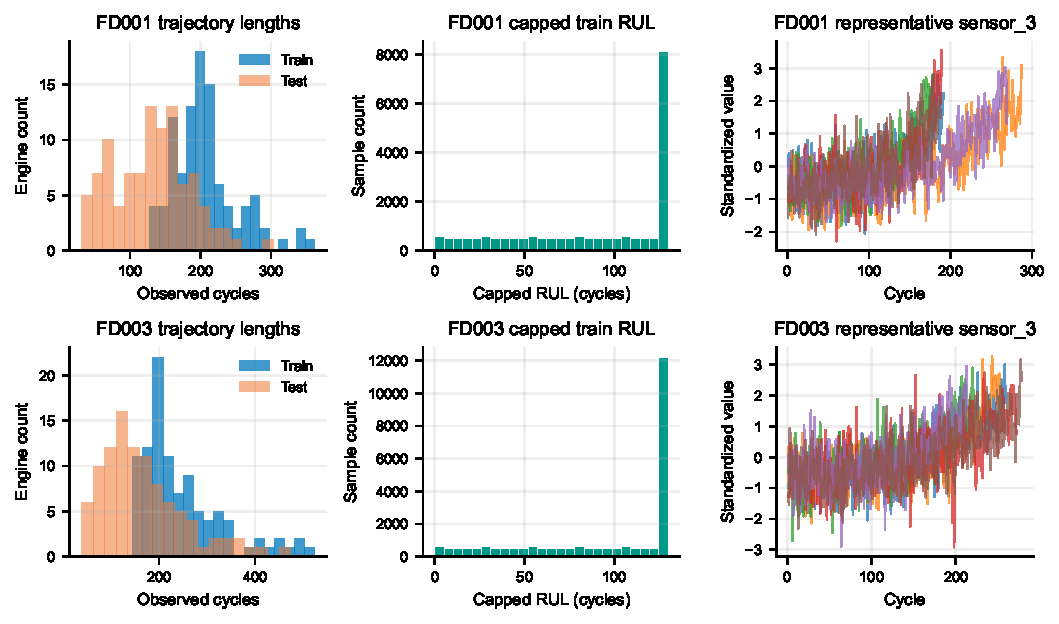
\includegraphics[width=0.98\textwidth]{figure_01_data_overview.pdf}
\caption{Data overview for FD001 and FD003. The figure reports train/test trajectory lengths, capped training RUL distribution, and representative standardized sensor-3 trajectories.}
\label{fig:data-overview}
\end{figure*}

\subsection{Overall Model Comparison}

Table~\ref{tab:main-results} summarizes selected complete three-seed test results, matching the settings visualized in Figure~\ref{fig:model-comparison}. On FD001, Gradient Boosting and Random Forest have the best aggregate RMSE among the evaluated models. The plain GRU and LSTM underperform those tree baselines in global RMSE, while the CNN configuration fails badly. On FD003, the GRU with a 50-cycle window obtains the numerically lowest RMSE among the evaluated configurations, narrowly ahead of Gradient Boosting. A paired bootstrap over seed--engine pairs gives an RMSE difference of $-0.25$ cycles for GRU window50 minus Gradient Boosting with a 95\% interval of $[-1.45, 1.00]$, so the apparent FD003 advantage should not be treated as statistically resolved.

\begin{table*}[t]
\centering
\caption{Selected complete three-seed test metrics on FD001 and FD003. RMSE is shown as mean $\pm$ standard deviation over three seeds. Lower is better for RMSE, MAE, NASA score, critical RMSE, and overestimation ratio.}
\label{tab:main-results}
\small
\begin{tabular}{llrrrr}
\toprule
Subset & Model & RMSE & MAE & NASA score & RMSE$_{50}$ / OverRatio \\
\midrule
FD001 & Gradient Boosting & $12.81\pm0.38$ & 9.83 & 247.46 & 5.60 / 0.607 \\
FD001 & Random Forest & $13.01\pm0.57$ & 9.62 & 258.65 & 6.21 / 0.617 \\
FD001 & GRU safety-w1.5 & $13.99\pm0.26$ & 10.01 & 312.82 & 4.94 / 0.563 \\
FD001 & GRU safety-w2 & $14.96\pm0.88$ & 10.59 & 421.19 & 4.86 / 0.467 \\
FD001 & GRU & $15.27\pm0.64$ & 11.33 & 483.23 & 5.71 / 0.587 \\
FD001 & LSTM & $15.60\pm0.51$ & 11.45 & 563.57 & 6.52 / 0.627 \\
FD001 & GRU window50 & $15.67\pm0.58$ & 11.65 & 425.21 & 6.13 / 0.523 \\
FD001 & Ridge & $16.92\pm0.11$ & 13.33 & 510.32 & 16.68 / 0.580 \\
FD001 & 1D-CNN & $22.47\pm1.17$ & 16.49 & 3867.77 & 25.42 / 0.563 \\
\midrule
FD003 & GRU window50 & $12.96\pm0.48$ & 9.30 & 319.96 & 5.50 / 0.533 \\
FD003 & Gradient Boosting & $13.21\pm0.35$ & 9.67 & 311.85 & 5.53 / 0.573 \\
FD003 & Random Forest & $13.98\pm0.25$ & 10.14 & 343.90 & 4.76 / 0.583 \\
FD003 & GRU safety-w1.5 & $14.07\pm1.24$ & 9.96 & 413.74 & 5.25 / 0.437 \\
FD003 & LSTM & $14.41\pm1.57$ & 10.22 & 550.26 & 5.09 / 0.507 \\
FD003 & GRU & $15.24\pm1.45$ & 10.55 & 622.27 & 6.19 / 0.553 \\
FD003 & GRU safety-w2 & $15.99\pm2.61$ & 11.99 & 608.31 & 7.57 / 0.430 \\
FD003 & Ridge & $18.02\pm0.37$ & 14.90 & 627.31 & 15.87 / 0.600 \\
FD003 & 1D-CNN & $23.76\pm0.42$ & 17.25 & 3533.32 & 24.91 / 0.570 \\
\bottomrule
\end{tabular}
\end{table*}

Figure~\ref{fig:model-comparison} visualizes RMSE with seed variability for the same selected complete configurations. It reinforces that tree ensembles are strong FD001 baselines and that longer temporal context is promising for the GRU on FD003, while the bootstrap interval above keeps that comparison appropriately cautious.

\begin{figure*}[t]
\centering
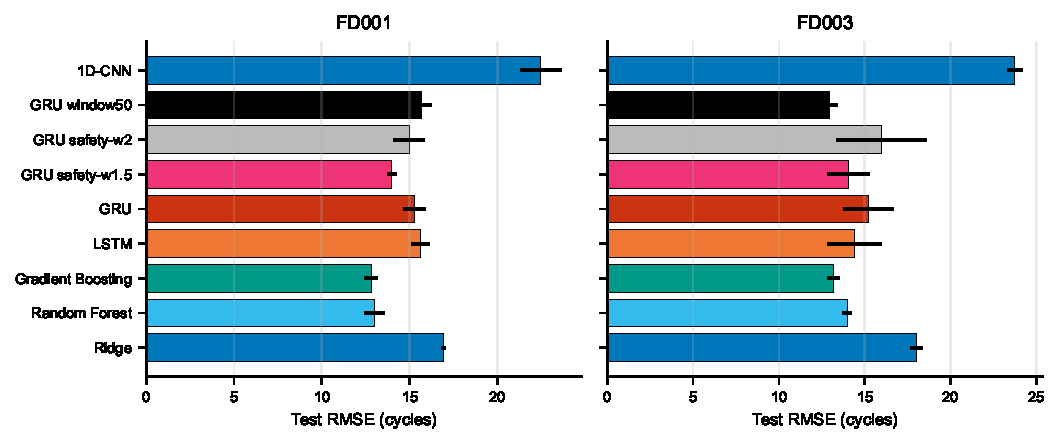
\includegraphics[width=0.98\textwidth]{figure_02_model_comparison.pdf}
\caption{Aggregate RMSE comparison. Error bars indicate standard deviation over completed seeds where available.}
\label{fig:model-comparison}
\end{figure*}

\subsection{Prediction Calibration and Residual Behavior}

Figure~\ref{fig:prediction-scatter} compares predicted and true RUL for representative FD001 and FD003 models. Prediction scatter reveals structure that table metrics hide: models can be accurate for many mid-life engines while still producing dangerous optimistic outliers near low true RUL.

\begin{figure*}[t]
\centering
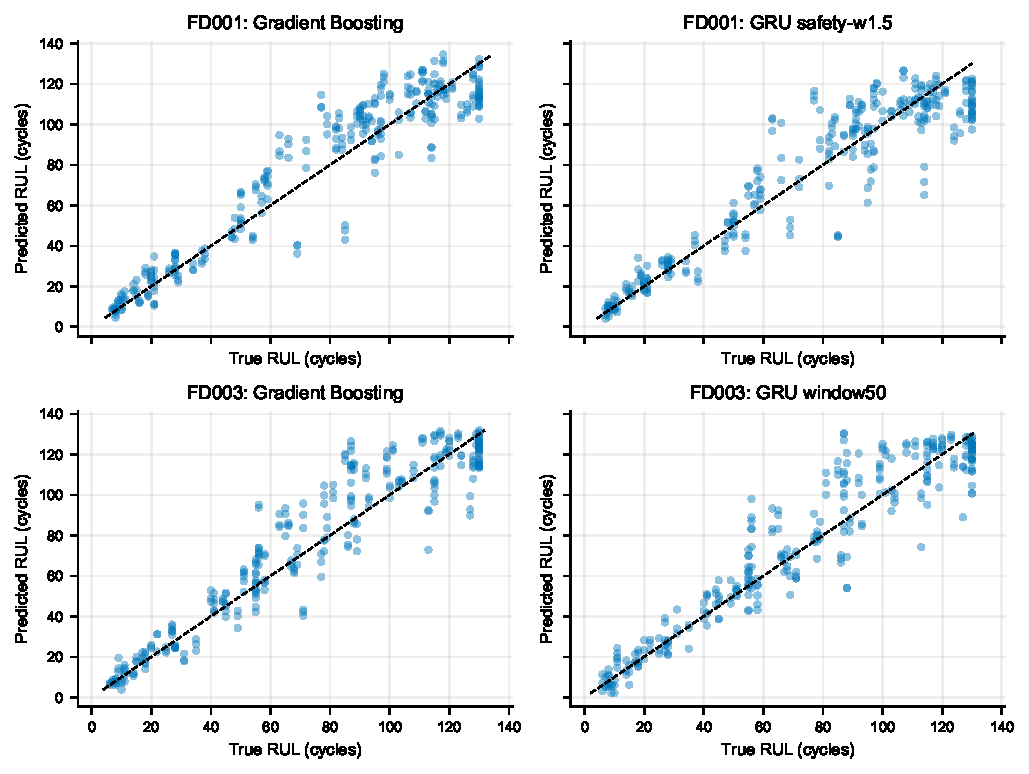
\includegraphics[width=0.95\textwidth]{figure_03_predicted_vs_true.pdf}
\caption{Predicted versus true RUL for representative models. The dashed line marks perfect prediction. Points above the line overestimate RUL.}
\label{fig:prediction-scatter}
\end{figure*}

Figure~\ref{fig:critical-residuals} separates residuals inside and outside the $y\leq50$ critical zone. This is the central safety diagnostic. On FD001, safety-weighted GRUs improve critical-zone RMSE relative to the plain GRU and tree models, although they do not beat Gradient Boosting on aggregate RMSE. On FD003, stronger safety weighting reduces overestimation frequency but can worsen RMSE and critical-zone RMSE, exposing a real accuracy--conservatism trade-off.

\begin{figure*}[t]
\centering
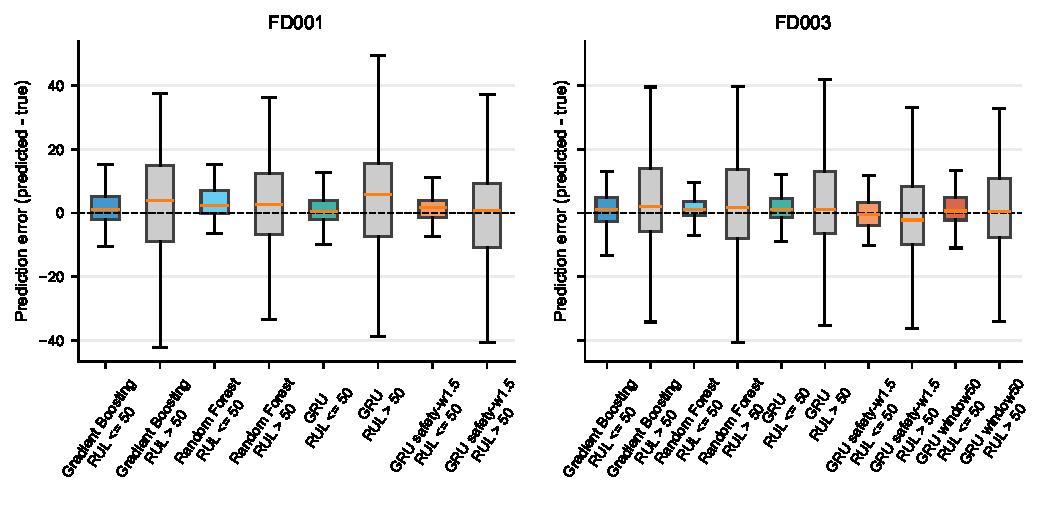
\includegraphics[width=0.98\textwidth]{figure_04_critical_residuals.pdf}
\caption{Residual distributions inside and outside the critical zone. Positive residuals indicate RUL overestimation.}
\label{fig:critical-residuals}
\end{figure*}

\subsection{Engine-Level Failure Cases}

RUL evaluation should also inspect which engines are difficult. Figure~\ref{fig:hardest-engines} shows the highest mean absolute error units for representative models. These engine-level diagnostics are useful for identifying whether a model fails on isolated trajectories or exhibits a systematic subset-level weakness.

\begin{figure*}[t]
\centering
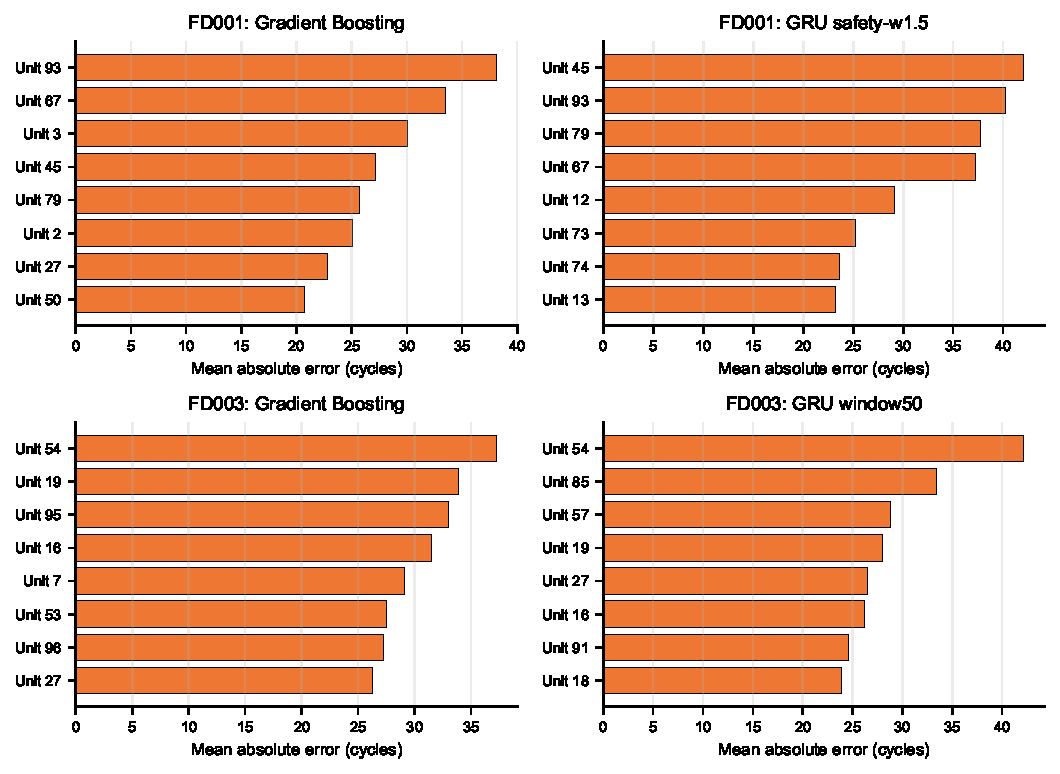
\includegraphics[width=0.95\textwidth]{figure_05_hardest_engines.pdf}
\caption{Hardest test engines by mean absolute error. Values are aggregated across available seeds for each model setting.}
\label{fig:hardest-engines}
\end{figure*}

\subsection{Safety Trade-Offs}

Figure~\ref{fig:safety-tradeoff} plots overestimation ratio against critical-zone RMSE. The ideal direction is lower-left. The key observation is that model ranking changes across safety axes. Random Forest has the best FD003 critical RMSE, Gradient Boosting has strong aggregate performance, GRU window50 has the numerically lowest FD003 RMSE, and safety-w2 has the lowest FD003 overestimation ratio among complete three-seed configurations.

\begin{figure*}[t]
\centering
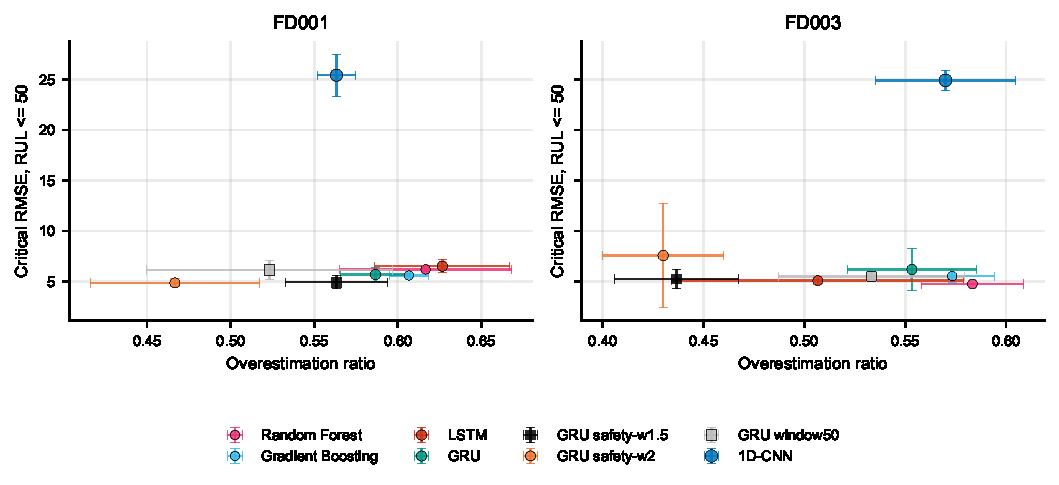
\includegraphics[width=0.95\textwidth]{figure_06_safety_tradeoff.pdf}
\caption{Safety trade-off between overestimation frequency and critical-zone RMSE. Circles mark main benchmark models and squares mark focused GRU variants. Error bars show seed variability when available.}
\label{fig:safety-tradeoff}
\end{figure*}

\subsection{Deep Training Dynamics and Feature Importance}

Figure~\ref{fig:learning-curves} shows validation losses for deep models. The CNN's poor test behavior is consistent with unstable or less effective optimization under the current compact architecture and training budget. Extending epochs alone is therefore not a principled fix; architecture, window length, loss weighting, and regularization matter more.

\begin{figure*}[t]
\centering
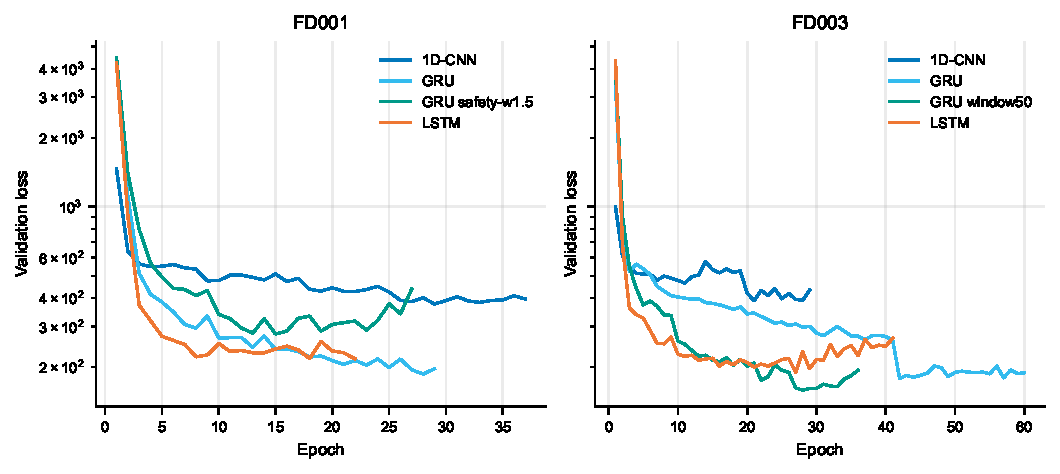
\includegraphics[width=0.98\textwidth]{figure_07_learning_curves.pdf}
\caption{Validation-loss trajectories for deep models. Curves are averaged over available seeds for each setting.}
\label{fig:learning-curves}
\end{figure*}

For tree models, Figure~\ref{fig:feature-importance} shows Random Forest feature importance. Important features often include mean and slope terms, supporting the intuition that both degradation level and trend carry RUL information.

\begin{figure*}[t]
\centering
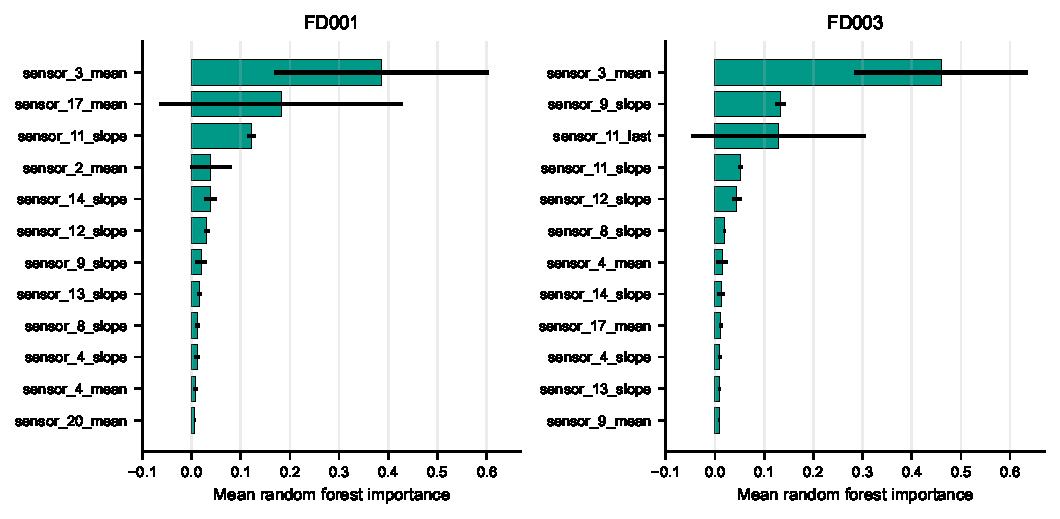
\includegraphics[width=0.95\textwidth]{figure_08_feature_importance.pdf}
\caption{Random Forest feature importance summarized across seeds. Mean and slope statistics are frequently important, suggesting that both current degradation level and temporal trend matter.}
\label{fig:feature-importance}
\end{figure*}

\clearpage

\section{Discussion}

\subsection{Classical Baselines Remain Strong}

The FD001 results show that a well-constructed feature-engineered tree baseline can outperform basic deep models. This is an important lesson for student research: using an LSTM does not automatically make the method stronger. When the dataset is small and the operating condition is simple, tabular summaries can capture enough degradation information for tree ensembles to be highly competitive.

\subsection{Temporal Context Helps More on FD003}

FD003 introduces two fault modes while keeping one operating condition. In this setting, the 50-cycle GRU improves substantially over the default 30-cycle GRU and has the numerically lowest mean RMSE. However, the paired bootstrap interval against Gradient Boosting crosses zero, so this result supports only a cautious interpretation: longer temporal context may help recurrent models when degradation patterns become more heterogeneous, but the current evidence does not establish a statistically resolved advantage over the tree baseline.

\subsection{Safety-Aware Training Changes the Error Profile}

The safety-aware GRU is not globally best, but it shifts behavior in a useful direction. On FD001 it improves critical-zone RMSE, especially under stronger safety weighting. On FD003 it reduces overestimation ratio, but the w2 setting also worsens RMSE and critical-zone RMSE. These outcomes match the intended purpose of the experiment: changing the risk profile rather than simply minimizing average squared error. A stronger future method could directly optimize differentiable approximations of NASA score or use calibration-aware post-processing.

\subsection{Why the CNN Fails Here}

The CNN configuration performs poorly on both subsets. This should not be interpreted as evidence that CNNs are unsuitable for RUL prediction in general, since stronger CNN designs have been reported \citep{Babu2016,Li2018}. The local explanation is more modest: the current compact CNN and training setup do not extract robust degradation features from the available windows. This failure is still useful because it shows why benchmark papers should include diagnostic curves and not only final scores.

\section{Threats to Validity}

\textbf{Internal validity.} The pipeline controls common leakage risks through engine-level validation splitting and train-only scaler fitting. Remaining internal risks include hyperparameter budget imbalance, stochastic training variability, and incomplete coverage of some wide-sweep ablation cells.

\textbf{Construct validity.} RMSE, MAE, NASA score, critical-zone RMSE, and overestimation ratio are proxies for prognostic usefulness. They do not validate a real maintenance decision policy. The safety-aware loss is a simple benchmark intervention, not a certified safety mechanism.

\textbf{External validity.} FD001 and FD003 are simulated single-operating-condition subsets. Results may not transfer to FD002/FD004, real engine fleets, multi-condition normalization settings, or engines with different sensor suites.

\section{Limitations and Future Work}

This work is intentionally scoped. It does not claim state-of-the-art performance, does not tune every model equally, and does not validate on real aircraft engine data. Future work should add FD002/FD004, stronger CNN and attention baselines, differentiable score-based losses, prediction interval calibration, broader paired statistical comparisons, and a clearer model-selection policy under asymmetric maintenance costs.

\section{Conclusion}

This paper upgrades a C-MAPSS RUL benchmark from a simple model comparison to a safety-aware evaluation study. The main finding is not that one architecture universally wins. Instead, tree ensembles are strong on FD001, longer-window GRUs are promising on FD003, and safety-aware loss can reduce late-life or overestimation risk while sometimes sacrificing aggregate accuracy. For C-MAPSS RUL research, RMSE alone is not enough; critical-zone error and overestimation behavior should be part of the standard reporting package.

\section*{Data and Code Availability}

The raw C-MAPSS data are available from the NASA Prognostics Center of Excellence repository \citep{NASA_PCoE} and are not redistributed in this repository. Code, experiment scripts, generated tables, figures, LaTeX source, and the arXiv source package are available at:
\url{https://github.com/EthanHuangEbor/Cmaps_RULE}. The intended reproducibility tag for this draft is \texttt{arxiv-draft-2026-06-25}.

\section*{Ethics, Funding, Conflicts, and AI Disclosure}

This study uses a public simulation benchmark and does not involve human participants, animals, or proprietary operational data. The author reports no external funding and no conflicts of interest. AI assistance was used for coding support, manuscript drafting, figure-generation planning, and reviewer-style critique. The author remains responsible for all claims, code, experimental interpretation, and final submission decisions.

\section*{Author Contributions}

Ethan Huang designed the study, ran and interpreted the experiments, maintained the repository, and prepared the manuscript with AI-assisted drafting and review support.

\bibliographystyle{unsrtnat}
\bibliography{references}

\end{document}
